%% The first command in your LaTeX source must be the \documentclass command.
%%
%% Options:
%% twocolumn : Two column layout.
%% hf: enable header and footer.
\documentclass[
% twocolumn,
% hf,
]{ceurart}

%%
%% One can fix some overfulls
\sloppy

%%
%% Minted listings support 
%% Need pygment <http://pygments.org/> <http://pypi.python.org/pypi/Pygments>
\usepackage{minted}
%% auto break lines
% \lstset{breaklines=true}

%%
%% end of the preamble, start of the body of the document source.
\newcommand{\email}[1]{\texttt{#1}}
\graphicspath{{pics/}}

\begin{document}

%%
%% Rights management information.
%% CC-BY is default license.
%\copyrightyear{2022}
% \copyrightclause{Copyright for this paper by its authors.  Use permitted under Creative Commons License Attribution 4.0  International (CC BY 4.0).}

%%
%% This command is for the conference information
\conference{AIIT'2022
14 October, 2022, Zrenjanin, Serbia}

%%
%% The "title" command
\title{Using knowledge graph based distributed infrastructure for processing educational documents}
% Менять можно все, и заголовок.... мы тут сами по себе

%%
%% The "author" command and its associated commands are used to define
%% the authors and their affiliations.
\author[1,2]{Evgeny A. Cherkashin}
\author[2]{Victoria A. Popova}
% \cormark[1]
% \fnmark[1]
\address[1]{Matrosov Institute for System Dynamics and Control Theory SB RAS, Irkutsk, Russia}
\address[2]{Institute of Mathematics and Information Technologies, Irkutsk State University, Irkutsk, Russia\\[0.7em]
\email{eugeneai@icc.ru};\quad\email{victorypopova1@gmail.com}}

%% Footnotes
% \cortext[1]{Corresponding author.}
%\fntext[1]{These authors contributed equally.}

%%
%% The abstract is a short summary of the work to be presented in the
%% article.
\begin{abstract}
  This paper deals with the application of early developed infrastructural components based on knowledge graph data representation and knowledge-based data processing to university course documents processing, authoring and providing with their data a future platform for organization of the educational process.  
  
  Main goal of the activity is to integrate static university facade data represented as educational program documentation with university infrastructure, e.g., library, schedule, various existing process planning systems already made by master students and university staff.
\end{abstract}

%%
%% Keywords. The author(s) should pick words that accurately describe
%% the work being presented. Separate the keywords with commas.
\begin{keywords}
  knowledge graph \sep
  logical inference \sep
  education process automation \sep
  distributed data processing
\end{keywords}

%%
%% This command processes the author and affiliation and title
%% information and builds the first part of the formatted document.
\maketitle
%     July 2020

% DOI:10.47350/ICCS-DE.2020.24
%    Proceedings of The International Workshop on Information, Computation, and Control Systems for Distributed Environments

\section{Introduction}

University is a complex socio-technical system (STS) \cite{zh2020} comprising various components, which functioning is provided mostly by university staff and automation software.  Irkutsk state university (ISU) has quite normal (required) level of automation in the areas of accounting, education process planning, learning management, student state control, library data access with library information system (LIS).  The automation has an island character between areas of automation and institutions (institutes and their departments).  Some institutes of ISU develop localized software to solve their own problems and do not share results between ISU community, or adaptation efforts assessed as senseless. It seems that there is no such tradition.  Some solutions are implemented by a special department of Institute of Mathematics and Information Technologies (IMIT) of ISU on a request.  For example, during COVID-19 pandemics, IMIT supported Big blue button functioning for all departments of ISU, implemented Moodle modules for remote enrollment management.

% syllabus - sillabi (pl.) = Рабочая прграмма дисциплины.
% curriculum - curricula (pl.) = учебный план.
% faculty - профессорско-преподавательский состав (ППС)

To obey constantly rising requirements placed on a university functioning, some areas are still experiencing a lack of automation. One of the challenging problem is course documentation, such as syllabi, mediation with a curriculum. In a syllabus, in the case of contracting or changing the numbers of hours spent to lecture and laboratory works, teacher must reschedule the amounts by adding/removing topics or contracting/extending a topic content.  {\bf[Другой пример непростой задачи ДОБАВИТЬ]} The format of printing layout of the syllabi is altered every two years, and even unchanged content must be reconstructed.  Yet another task that has not yet been automated is to check the capabilities of the university library to supply printing editions for references of the syllabi, renew URL references to the electronic ones.  Another problem deals with educational process management.  There is no common system of class schedule planning and browsing, monitoring student progress, namely, the fact of attending a class and the obtained grades.  % Some departments have their localized solutions, which cannot be efficiently adapted.
% Другой проблемой, которую требуется решить непосредственно по части организации учебного процесса, является отсутствие единой информационной системы, которая бы позволила просматривать расписание занятий, а также контролировать успеваемость студентов за счёт выставления оценок и отметок о посещаемости занятий. Важно отметить, что некоторыми учебными подразделениями такие проблемы уже решены. Но разработанные информационные системы адаптированы под характеристики конкретного учебного подразделения, что не позволяет использовать ту же систему в другом подразделении. Поэтому требуются такие программные продукты, которые могли бы использовать все институты и факультеты ИГУ для решения проблем организации учебного процесса.

The abovementioned problems are solved by faculty manually using office automation software (Microsoft and LibreOffice), institute management staff develop recommendations and template documents to simplify and inspire faculty to proceed with authoring of the syllabi in time and result in a good quality documents (in all aspects).  The devised manually, class schedules are published on ISU site as soon as they formed.  In such circumstances, its reconstruction becomes inoperative.   %  Что касается задач представления расписания и контроля успеваемости студентов, такие задачи также часто решаются вручную при помощи продуктов Microsoft и LibreOffice, из-за чего  редактирование расписания занятий является неоперативным процессом, поскольку изменения будут отображаться студентам и преподавателям только после публикации документа на веб-сайте или на стенде института. При достаточном количестве человеческих ресурсов такого вида работы могут быть выполнены оперативно с низкой вероятностью возникновения ошибок.  
The human factor is exposed in a degradation of the quality of requirements compliance.  This is, partially, due to the present underestimation of the role of a teacher and economic reasons: teachers often have positions in other institutions and mentally not interesting in placing this activity to the first place in their everyday schedule.

It seems that the problems can be solved by using artificial intelligence at a good level.  ISU site includes units for supplying students and faculty with the educational process documents, including curricula and syllabi for the past few years for all study programs.  Documents are represented in PDF format and can be informative sources of meaningful data, as well as various documents from Russian government sites containing references books for specialities, job requirements, {\em etc}. 

Other two abovementioned problems of class scheduling and student progress monitoring have many aspects of consideration, including use of combinatorial optimization engines for solving constraint satisfaction problem of scheduling, data representation for students' grades (formal and instructive), their meaningful description, compliance to educational trajectories, competence set, creative solutions, and formal tests.

% Это слишко детально для введения. Но дает мне понимание проблематики. Я не выкидываю твой труд, просто резюмирую.
%Проблемы автоматизации представления расписания и контроля успеваемости также являются решаемыми задачами, хоть и далеко не простыми. На текущий момент во многих учебных подразделениях ИГУ расписание предоставляется только в файле Word или Excel. В таких файлах расписание занятий сортируется по студенческим группам, что влечёт трудности поиска занятий преподавателем. Расписание такого формата также неудобно просматривать с мобильных устройств. Стоит отметить, что во всех учебных подразделениях ИГУ расписание отличается своим представлением, поэтому при разработке системы требуется учитывать настраивающийся интерфейс, чтобы студенты и преподаватели не испытывали трудностей при просмотре расписания  и быстро привыкли к использованию приложений для расписания. 

% Для контроля успеваемости студентов также требуется система, которая бы позволяла добавлять оценки как в течение учебного семестра за занятия, так и предназначалась для ввода данных об зачётах, экзаменах, курсовых работах и практиках. Немаловажно учитывать и посещаемость занятий студентами. Чаще всего такие данные заполняются преподавателем на обычном бумажном листе, информация с которого может далее быть перенесена вручную на электронные устройства для, например, расчёта в программе Excel оценки или суммы баллов за учебный семестр. 

The aim of the present research presented in the paper is to automate these creative activities of the faculty authoring syllabi, organizing processes, monitoring and control, and in the future, form a basis of educational process modelling to support the compliance checking, individual education trajectories of students, compliance to domain of courses.

\section{Short description of the platform}

The basis of the proposed and by component evaluation tested is usage of a common distributed warehousing driven by present semantic data servers, knowledge graph (KG) servers, such as Virtouso, ClioPatria, and adapting rational databases to Semantic Web (SW) technologies.  The usage of the distributed KGs allows us to develop subsystems independently, having in mind their facilities of coupling distributed data and services within common domains in a distributed network.  Using KG as data structures enables a developer to create software complexes as interacting agents via KGs' content, reaching loose coupling between them.  Another advantage of SW and KG usage is nowadays domain standardized descriptions represented as well-known vocabularies.  In Figure~\ref{fig:arch}

\begin{figure}
\centering
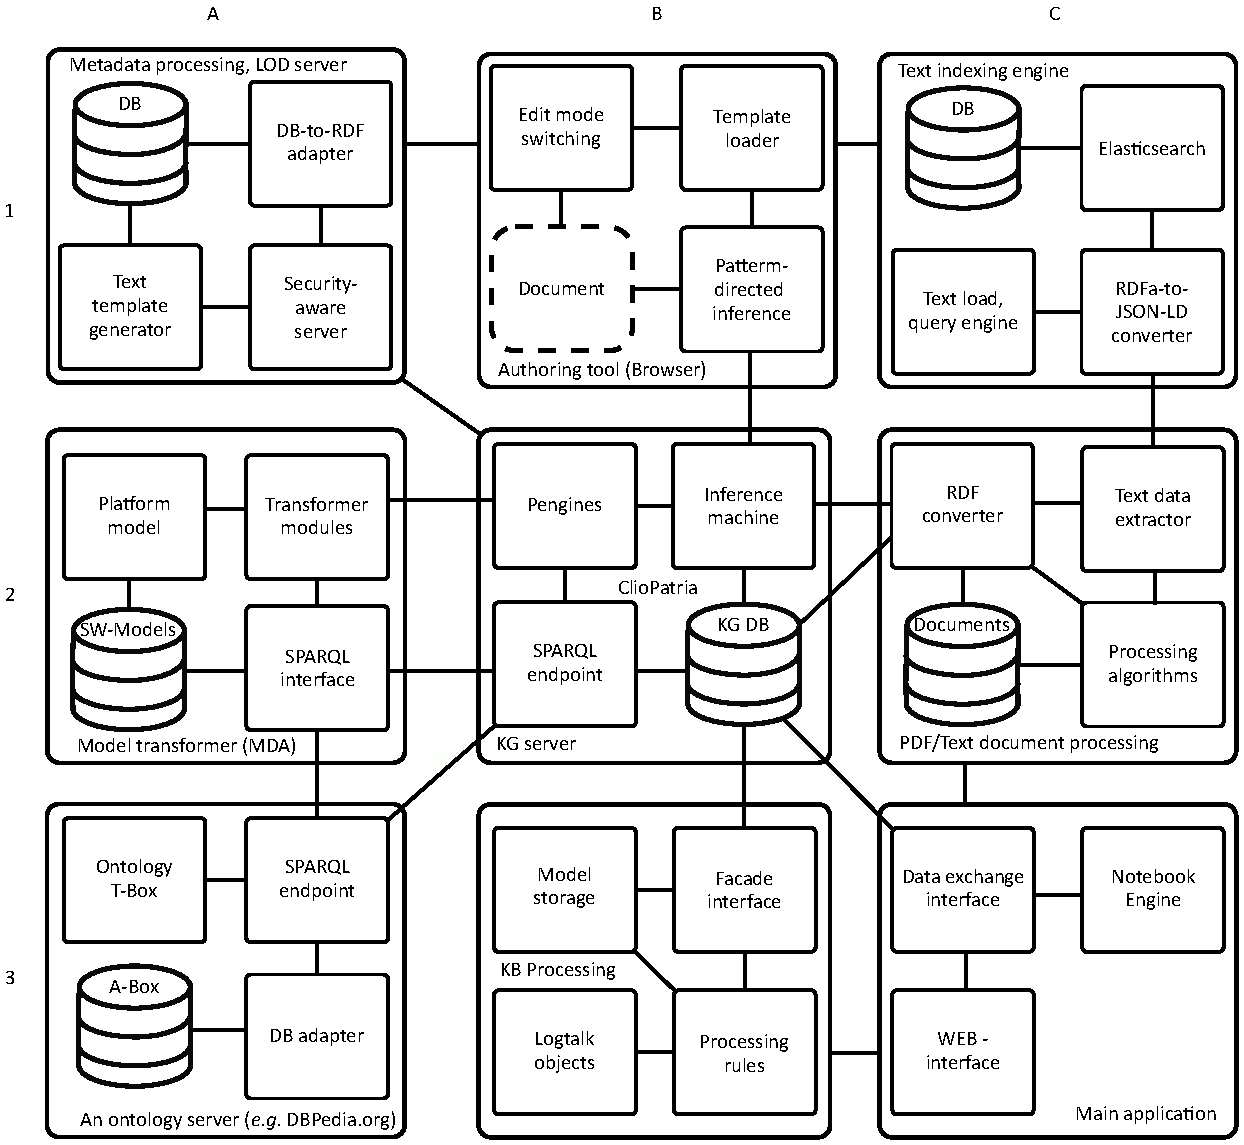
\includegraphics[width=1\linewidth]{architecture-mda-lod-ext-general.pdf}
\caption{General archiceture of KG based software development platform}
\label{fig:arch}
\end{figure}

\section{A general idea of the infrastructure application}

Modifying the template --- including but not limited to: adjusting
margins, typeface sizes, line spacing, paragraph and list definitions,
and the use of the \verb|\vspace| command to manually adjust the
vertical spacing between elements of your work --- is not allowed.

\section{Template parameters}

There are a number of template
parameters which modify some part of the \verb|ceurart| document class.
This parameters are enclosed in square
brackets and are a part of the \verb|\documentclass| command:


Frequently-used parameters, or combinations of parameters, include:
\begin{itemize}
\item \verb|twocolumn| : Two column layout.
\item \verb|hf| : Enable header and footer\footnote{You can enable
    the display of page numbers in the final version of the entire
    collection. In this case, you should adhere to the end-to-end
    pagination of individual papers.}.
\end{itemize}

\section{Front matter}

\subsection{Title Information}

The titles of papers should be either all use the emphasizing
capitalized style or they should all use the regular English (or
native language) style. It does not make a good impression if you or
your authors mix the styles.

Use the \verb|\title| command to define the title of your work. Do not
insert line breaks in your title.

\subsection{Title variants}


\subsection{Authors and Affiliations}

Each author must be defined separately for accurate metadata
identification. Multiple authors may share one affiliation. Authors'
names should not be abbreviated; use full first names wherever
possible. Include authors' e-mail addresses whenever possible.

\verb|\author| command have the below options: 

\begin{itemize}
\item \verb|style| : Style of author name (chinese)
\item \verb|prefix| : Prefix
\item \verb|suffix| : Suffix
\item \verb|degree| : Degree
\item \verb|role| : Role
\item \verb|orcid| : ORCID
\item \verb|email| : E-mail
\item \verb|url| : URL
\end{itemize}

Author names can have some kinds of marks and notes:
\begin{itemize}
\item affiliation mark: \verb|\author[<num>]|.
\end{itemize}

The author names and affiliations could be formatted in two ways:
\begin{enumerate}
\item Group the authors per affiliation.
\item Use an explicit mark to indicate the affiliations.
\end{enumerate}

Author block example:


\subsection{Abstract and Keywords}

Abstract shall be entered in an environment that starts
with \verb|\begin{abstract}| and ends with
\verb|\end{abstract}|. 



The key words are enclosed in a \verb|keywords|
environment. Use \verb|\sep| to separate keywords.



At the end of front matter add \verb|\maketitle| command.

\subsection{Various Marks in the Front Matter}

The front matter becomes complicated due to various kinds
of notes and marks to the title and author names. Marks in
the title will be denoted by a star ($\star$) mark;
footnotes are denoted by super scripted Arabic numerals,
corresponding author by an Conformal asterisk (*) mark.

\subsubsection{Title marks}

Title mark can be entered by the command, \verb|\tnotemark[<num>]|
and the corresponding text can be entered with the command
\verb|\tnotetext[<num>]{<text>}|. An example will be:



\verb|\tnotemark| and \verb|\tnotetext| can be anywhere in
the front matter, but should be before \verb|\maketitle| command.

\subsubsection{Author marks}

Author names can have some kinds of marks and notes:
\begin{itemize}
\item footnote mark : \verb|\fnmark[<num>]|
\item footnote text : \verb|\fntext[<num>]{<text>}|
\item corresponding author mark : \verb|\cormark[<num>]|
\item corresponding author text : \verb|\cortext[<num>]{<text>}|
\end{itemize}

\subsubsection{Other marks}

At times, authors want footnotes which leave no marks in
the author names. The note text shall be listed as part of
the front matter notes. Class files provides
\verb|\nonumnote| for this purpose. The usage

and should be entered anywhere before the \verb|\maketitle|
command for this to take effect. 

\section{Sectioning Commands}

Your work should use standard \LaTeX{} sectioning commands:
\verb|\section|, \verb|\subsection|,
\verb|\subsubsection|, and
\verb|\paragraph|. They should be numbered; do not remove
the numbering from the commands.

Simulating a sectioning command by setting the first word or words of
a paragraph in boldface or italicized text is not allowed.

\section{Tables}

The ``\verb|ceurart|'' document class includes the ``\verb|booktabs|''
package --- \url{https://ctan.org/pkg/booktabs} --- for preparing
high-quality tables.

Table captions are placed \textit{above} the table.

Because tables cannot be split across pages, the best placement for
them is typically the top of the page nearest their initial cite.  To
ensure this proper ``floating'' placement of tables, use the
environment \verb|table| to enclose the table's contents and the
table caption. The contents of the table itself must go in the
\verb|tabular| environment, to be aligned properly in rows and
columns, with the desired horizontal and vertical rules.

Immediately following this sentence is the point at which
Table~\ref{tab:freq} is included in the input file; compare the
placement of the table here with the table in the printed output of
this document.

\begin{table*}
  \caption{Frequency of Special Characters}
  \label{tab:freq}
  \begin{tabular}{ccl}
    \toprule
    Non-English or Math&Frequency&Comments\\
    \midrule
    \O & 1 in 1,000& For Swedish names\\
    $\pi$ & 1 in 5& Common in math\\
    \$ & 4 in 5 & Used in business\\
    $\Psi^2_1$ & 1 in 40,000& Unexplained usage\\
  \bottomrule
\end{tabular}
\end{table*}

To set a wider table, which takes up the whole width of the page's
live area, use the environment \verb|table*| to enclose the table's
contents and the table caption.  As with a single-column table, this
wide table will ``float'' to a location deemed more
desirable. Immediately following this sentence is the point at which
Table~\ref{tab:commands} is included in the input file; again, it is
instructive to compare the placement of the table here with the table
in the printed output of this document.

\begin{table}
  \caption{Some Typical Commands}
  \label{tab:commands}
  \begin{tabular}{ccl}
    \toprule
    Command &A Number & Comments\\
    \midrule
    \texttt{{\char'134}author} & 100& Author \\
    \texttt{{\char'134}table}& 300 & For tables\\
    \texttt{{\char'134}table*}& 400& For wider tables\\
    \bottomrule
  \end{tabular}
\end{table}

\section{Math Equations}

You may want to display math equations in three distinct styles:
inline, numbered or non-numbered display.  Each of the three are
discussed in the next sections.

\subsection{Inline (In-text) Equations}

A formula that appears in the running text is called an inline or
in-text formula.  It is produced by the \verb|math| environment,
which can be invoked with the usual
\verb|\begin| \ldots \verb|\end| construction or with
the short form \verb|$| \ldots \verb|$|. You can use any of the symbols
and structures, from $\alpha$ to $\omega$, available in
\LaTeX~\cite{Lamport:LaTeX};
this section will simply show a few
examples of in-text equations in context. Notice how this equation:
\begin{math}
  \lim_{n\rightarrow \infty} \frac{1}{n} = 0,
\end{math}
set here in in-line math style, looks slightly different when
set in display style.  (See next section).

\subsection{Display Equations}

A numbered display equation---one set off by vertical space from the
text and centered horizontally---is produced by the \verb|equation|
environment. An unnumbered display equation is produced by the
\verb|displaymath| environment.

Again, in either environment, you can use any of the symbols and
structures available in \LaTeX{}; this section will just give a couple
of examples of display equations in context.  First, consider the
equation, shown as an inline equation above:
\begin{equation}
  \lim_{n\rightarrow \infty} \frac{1}{n} = 0.
\end{equation}
Notice how it is formatted somewhat differently in
the \verb|displaymath|
environment.  Now, we'll enter an unnumbered equation:
\begin{displaymath}
  S_{n} = \sum_{i=1}^{n} x_{i} ,
\end{displaymath}
and follow it with another numbered equation:
\begin{equation}
  \lim_{x \to 0} (1 + x)^{1/x} = e
\end{equation}
just to demonstrate \LaTeX's able handling of numbering.

\section{Figures}

The ``\verb|figure|'' environment should be used for figures. One or
more images can be placed within a figure. If your figure contains
third-party material, you must clearly identify it as such, as shown
in the example below.
\begin{figure}
  \centering
  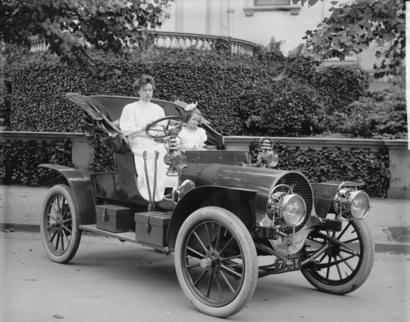
\includegraphics[width=\linewidth]{sample-franklin}
  \caption{1907 Franklin Model D roadster. Photograph by Harris \&
    Ewing, Inc. [Public domain], via Wikimedia
    Commons. (\url{https://goo.gl/VLCRBB}).}
\end{figure}

Your figures should contain a caption which describes the figure to
the reader. Figure captions go below the figure. Your figures should
also include a description suitable for screen readers, to
assist the visually-challenged to better understand your work.

Figure captions are placed below the figure.

\section{Citations and Bibliographies}

The use of Bib\TeX{} for the preparation and formatting of one's
references is strongly recommended. Authors' names should be complete
--- use full first names (``Donald E. Knuth'') not initials
(``D. E. Knuth'') --- and the salient identifying features of a
reference should be included: title, year, volume, number, pages,
article DOI, etc.

The bibliography is included in your source document with these two
commands, placed just before the \verb|\end{document}|
command:

where ``\verb|bibfile|'' is the name, without the ``\verb|.bib|''
suffix, of the Bib\TeX{} file.


\subsection{Some examples}

A paginated journal article \cite{Abril07}, an enumerated journal
article \cite{Cohen07}, a reference to an entire issue
\cite{JCohen96}, a monograph (whole book) \cite{Kosiur01}, a
monograph/whole book in a series (see 2a in spec. document)
\cite{Harel79}, a divisible-book such as an anthology or compilation
\cite{Editor00} followed by the same example, however we only output
the series if the volume number is given \cite{Editor00a} (so series
should not be present since it has no vol. no.), a chapter in a
divisible book \cite{Spector90}, a chapter in a divisible book in a
series \cite{Douglass98}, a multi-volume work as book \cite{Knuth97},
an article in a proceedings (of a conference, symposium, workshop for
example) (paginated proceedings article) \cite{Andler79}, a
proceedings article with all possible elements \cite{Smith10}, an
example of an enumerated proceedings article \cite{VanGundy07}, an
informally published work \cite{Harel78}, a doctoral dissertation
\cite{Clarkson85}, a master's thesis: \cite{anisi03}, an online
document / world wide web resource \cite{Thornburg01, Ablamowicz07,
  Poker06}, a video game (Case 1) \cite{Obama08} and (Case 2)
\cite{Novak03} and \cite{Lee05} and (Case 3) a patent
\cite{JoeScientist001}, work accepted for publication \cite{rous08},
prolific author \cite{SaeediMEJ10} and \cite{SaeediJETC10}. Other
cites might contain `duplicate' DOI and URLs (some SIAM articles)
\cite{Kirschmer:2010:AEI:1958016.1958018}. Multi-volume works as books
\cite{MR781536} and \cite{MR781537}. A couple of citations with DOIs:
\cite{2004:ITE:1009386.1010128,Kirschmer:2010:AEI:1958016.1958018}. Online
citations: \cite{TUGInstmem, Thornburg01, R, UMassCitations}.

\section{Acknowledgments}

Identification of funding sources and other support, and thanks to
individuals and groups that assisted in the research and the
preparation of the work should be included in an acknowledgment
section, which is placed just before the reference section in your
document.

This section has a special environment:
so that the information contained therein can be more easily collected
during the article metadata extraction phase, and to ensure
consistency in the spelling of the section heading.

Authors should not prepare this section as a numbered or unnumbered
\verb|\section|; please use the ``\verb|acknowledgments|'' environment.

\section{Appendices}

If your work needs an appendix, add it before the
``\verb|\end{document}|'' command at the conclusion of your source
document.

Start the appendix with the ``\verb|\appendix|'' command:

and note that in the appendix, sections are lettered, not
numbered. 

%%
%% The acknowledgments section is defined using the "acknowledgments" environment
%% (and NOT an unnumbered section). This ensures the proper
%% identification of the section in the article metadata, and the
%% consistent spelling of the heading.
\begin{acknowledgments}
  Thanks to the developers of ACM consolidated LaTeX styles
  \url{https://github.com/borisveytsman/acmart} and to the developers
  of Elsevier updated \LaTeX{} templates
  \url{https://www.ctan.org/tex-archive/macros/latex/contrib/els-cas-templates}.  
\end{acknowledgments}

%%
%% Define the bibliography file to be used
\bibliography{sample-ceur}

%%
%% If your work has an appendix, this is the place to put it.
\appendix

\section{Online Resources}


The sources for the ceur-art style are available via
\begin{itemize}
\item \href{https://github.com/yamadharma/ceurart}{GitHub},
% \item \href{https://www.overleaf.com/project/5e76702c4acae70001d3bc87}{Overleaf},
\item
  \href{https://www.overleaf.com/latex/templates/template-for-submissions-to-ceur-workshop-proceedings-ceur-ws-dot-org/pkfscdkgkhcq}{Overleaf
    template}.
\end{itemize}

\end{document}

%%
%% End of file
